\chapter{Inductancia}
\section{Inductancia mutua}

\begin{figure}[h]
\centering
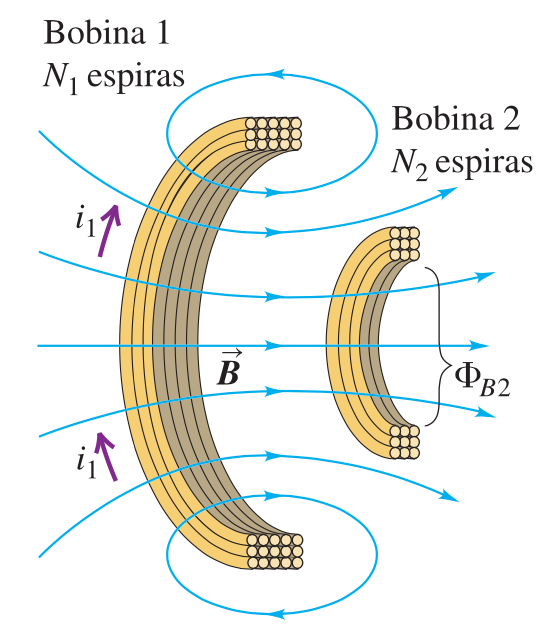
\includegraphics[scale=0.3]{fig/bobinas}
\caption{\textbf{Inductancia mutua}, si la corriente en la bobina 1 está cambiando, el flujo cambiante a través de la bobina 2 indice una fem en esta última}
\label{fig:bobinas}
\end{figure}
Interacción magnética entre dos alambres que trasnportan corrientes \textit{estables}; la corriente de uno de los alambres genera un campo magnético que ejerce una fuerza sobre la corriente entre el otro alambre. Cuando hay una corriente \textit{variable} en uno de los circuitos, surge una interacción adicional. Consideremos la situación de la figura
\ref{fig:bobinas}

Una corriente que circula por la bobina 1 produce un campo magnético $\vec{B}$ y, por lo tanto, un flujo magnético a través de la bobina 2. Si la corriente en la bobina 1 cambia, el flujo a través de la bobina 2 también cambia; de acuerdo con la ley de Faraday, esto induce una fem en la bobina 2. De este modo, un cambio en la corriente de un circuito puede inducir otra corriente en un segundo circuito.
Una corriente $i_1$\footnote{Denotamos con $i$ a una corriente variable en el tiempo } establece un campo magnético (indicado por las líneas de color azul), y algunas de estas líneas de campo pasan a través de la bobina 2. Denotaremos con $\Phi_{B2}$ el flujo magnético a través de \textit{cada} espira de la bobina 2, causado por la corriente $i_1$ en la bobina 1. (Si el flujo es diferente a través de las distintas espiras de la bobina, entonces $\Phi_{B2}$ denota el flujo  \textit{medio}). El campo magnético es proporcional a $i_1$, de manera que $\Phi_{B2}$ también es proporcional a $i_1$. \textbf{Cuando $i_1$ cambia, $\Phi_{B2}$ cambia; este flujo cambiante induce una fem $\varepsilon_2$ en la bobina 2}, dada por
\begin{equation}\label{fem}
\varepsilon_2=-N_2\frac{d\Phi_{B2}}{dt}
\end{equation}
Podríamos representar la proporcionalidad entre $\Phi_{B2}$ e $i_1$ en la forma $\Phi_{B2}$ = (constante) $i_1$, pero, en vez de ello, es más conveniente incluir el número de espiras $N_2$ en la relación. Al introducir una constante de proporcionalidad $M_{21}$, llamada \textbf{inductancia mutua} de las dos bobinas, escribimos
\begin{equation}\label{30.2}
N_2\Phi_{B2}=M_{21}i_1
\end{equation}
donde $\Phi_{B2}$ es el flujo a través de una sola espira de la bobina 2. De ahí que,
\begin{equation}
N_2\frac{d\Phi_{B2}}{dt}=M_{21}\frac{di_1}{dt}
\end{equation}
y la ecuación \ref{fem} se rescribe como
\begin{equation}
\varepsilon_2=-M_2\frac{di_1}{dt}
\end{equation}
Es decir, un cambio en la corriente $i_1$ en la bobina 1 induce una fem en la bobina 2, que es directamente proporcional a la tasa de cambio de $i_1$.

También se podría escribir la definición de la inductancia mutua, ecuación \ref{30.2}, como
\begin{equation}
M_{21}=\frac{N_2\Phi_{B2}}{i_1}
\end{equation}
\textbf{Si las bobinas están en el vacío}, el flujo $\Phi_{B2}$ a través de cada espira de la bobina 2 es directamente proporcional a la corriente $i_1$. Entonces, la inductancia mutua $M_{21}$ es una constante que sólo depende de la geometría de las dos bobinas.
Podría volverse a hacer el análisis para el caso opuesto, en el que una corriente cambiante $i_2$ en la bobina 2 causa un flujo cambiante $\Phi_{B}2$ y una fem $\varepsilon_1$ en la bobina 1. Se encuentra que, \textbf{$M_{12}$ siempre es igual a $M_{21}$, aun cuando las dos bobinas no sean simétricas}. A este valor común $M$ lo llamamos simplemente \textbf{inductancia mutua}. Por tanto, tenemos:
\begin{equation}\marginnote{Fem mutuamente inducidas}
\boxed{\varepsilon_2=-M\frac{di_1}{dt}\quad\mathrm{y}\quad \varepsilon_1=-M\frac{di_2}{dt}\quad}
\end{equation}
donde la inductancia mutua $M$ es
\begin{equation}\marginnote{Inductancia mutua}
\boxed{M=\frac{N_2\Phi_{B2}}{i_1}=\frac{N_1\Phi_{B1}}{i_2}}
\end{equation}
\textbf{Obs: Sólo una corriente variable en el tiempo induce una fem}.

La unidad del SI para la inductancia mutua se llama \textbf{henry} [$H$]
\section{Autoinductancia a inductores}
\begin{figure}[h]\label{fig:autoinductancia}
\centering
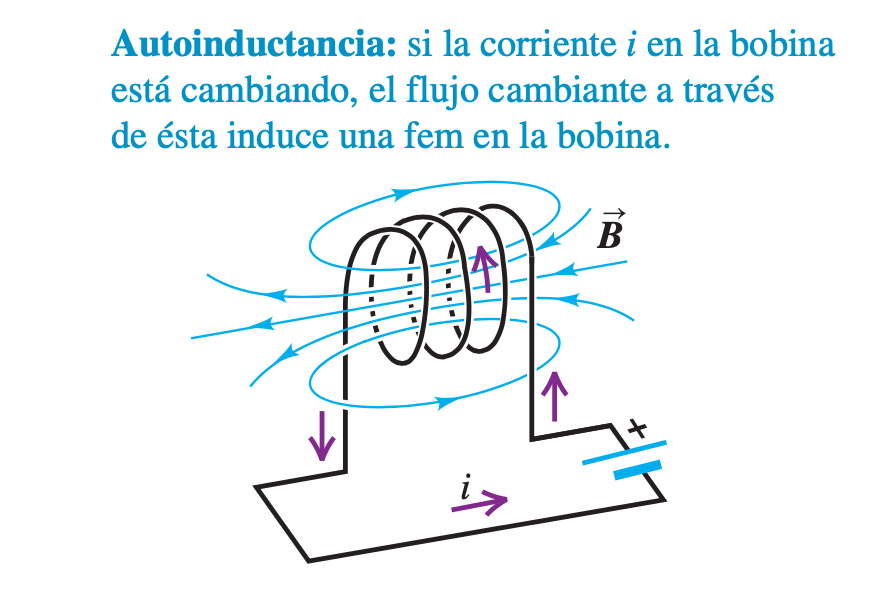
\includegraphics[scale=0.4]{fig/autoinductancia}
\caption{La corriente $i$ en el circuito crea un campo magnético $\vec{B}$ en la bobina y, por lo tanto, un flujo a través de ésta.}
\end{figure}

Consideremos un solo circuito aislado. Cuando en el circuito está presente una corriente, se establece un campo magnético que crea un flujo magnético a través del mismo circuito; este flujo cambia cuando la corriente cambia. Así, cualquier circuito que conduzca una corriente variable tiene una fem inducida en él por la variación en su propio campo magnético. Esa clase de fem se denomina \textbf{fem autoinducida}. Según la ley de Lenz, una fem autoinducida siempre se opone al cambio en la corriente que causó la fem, y de ese modo hace más difícil que haya variaciones en la corriente. El efecto se intensifica considerablemente si el circuito incluye una bobina con $N$ espiras de alambre. Como resultado de la corriente $i$, hay un flujo magnético medio $\Phi_B$ a través de cada vuelta de la bobina, figura \ref{fig:autoinductancia}.

Definimos la \textbf{autoinductancia} como
\begin{equation}\label{30.6.autoinductancia}\marginnote{Autoinductancia}
\boxed{L=\frac{N\Phi_B}{i}}
\end{equation}
Si la corriente $i$ en el circuito cambia, también lo hace el flujo $\Phi_B$. De ecuación \ref{30.6.autoinductancia} $$N\frac{d\Phi_B}{dt}=L\frac{di}{dt}$$ Utilizando la ley de Faraday, ecuación \ref{29.4.Nfaraday}, la fem autoinducida es
\begin{equation}\label{30.7}\marginnote{Fem autoinducida}
\boxed{\varepsilon=-L\frac{di}{dt}}
\end{equation}

\subsection{Los inductores como elementos de un circuito}
Un elemento de circuito diseñado para tener una inductancia particular se llama \textbf{inductor, o bobina de autoinducción}. Su finalidad es oponerse a cualquier variación en la corriente a través del circuito. Un inductor en un circuito de corriente directa ayuda a mantener una corriente estable a pesar de las fluctuaciones en la fem aplicada; en un circuito de corriente alterna, un inductor tiende a suprimir las variaciones de la corriente que ocurran más rápido de lo deseado.

Al utilizar la ley de Kirchhoff a traves de una malla conductora se suman sus diferencias de potencial y se igualan a cero porque el campo eléctrico producido por las cargas distribuidas es \textit{conservativo} ($\vec{E_c}$). El campo eléctrico inducido magnéticamente dentro de las bobinas del inductor \textbf{no es conservativo} ($\vec{E_n}$).


\begin{figure}[h]\label{fig30.5.circuito}
\centering
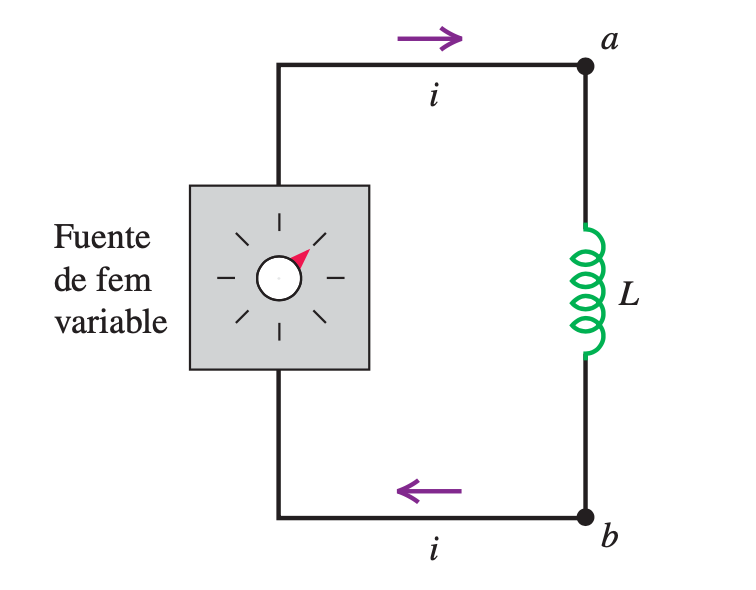
\includegraphics[scale=0.4]{fig/circuito}
\caption{Circuito que contiene una fuente de fem y un inductor. La fuente es variable, por lo que la corriente $i$ y su tasa de cambio $di>dt$ pueden variarse.}
\end{figure}

Consideremos el circuito de la figura \ref{fig30.5.circuito}. De acuerdo con la ley de Faraday, ecuación \ref{29.10}, la integral de línea de $\vec{E_n}$ alrededor del circuito es el negativo de la tasa de cambio del flujo a través del circuito. De ecuación \ref{30.7} $$\oint\vec{E_n}\cdot d\vec{l}=-L\frac{di}{dt}$$ donde se integra en sentido horario del circuito (el sentido supuesto para la corriente). Pero $\vec{E_n}$ es diferente de cero sólo dentro del inductor. Entonces $$\int_a^b\vec{E_n}\cdot d\vec{l}=-L\frac{di}{dt}$$ A continuación, como $\vec{E_c}+\vec{E_n}=0$ en cada punto dentro de las bobinas del inductor $$\int_a^b\vec{E_c}\cdot d\vec{l}=L\frac{di}{dt}$$ Pero esta integral es el potencial $V_{ab}$ del punto $a$ con respecto a $b$

\begin{equation}\label{30.8}
V_{ab}=V_a-V_b=L\frac{di}{dt}
\end{equation}

Se concluye que hay una diferencia de potencial genuina entre las terminales del inductor, asociada con las fuerzas conservativas electrostáticas, a pesar del hecho de que el campo eléctrico asociado con el efecto de inducción magnética es no conservativo.
\textbf{Obervación}: La fem autoinducida se opone a los cambios de la corriente ($di/dt$), \textit{no} a la corriente $i$ en sí.

\section{Energía del campo magnético}
El establecimiento de una corriente en un inductor requiere un suministro de energía, y un inductor que conduce corriente contiene energía almacenada. En la figura \ref{fig30.5.circuito}, una \textit{corriente creciente} $i$ ($di/dt>0$) en el inductor produce una fem $\varepsilon$ entre sus terminales, y una diferencia de potencial correspondiente $V_{ab}$ entre las terminales de la fuente, con el punto $a$ a mayor potencial que el $b$. Así, la fuente debe estar agregando energía al inductor, y la potencia instantánea $P$ (la tasa de transferencia de energía al inductor) es $P=V_{ab}i$.

\subsubsection{Energía almacenada en un inductor}
Si la corriente inicial es igual a cero, con la inductancia $L$ podemos calcular la entrada total de energía $U$ necesaria para establecer una corriente final $I$ en un inductor. Suponemos que el inductor tiene una resistencia igual a cero, por lo que dentro del inductor no se disipa energía. El voltaje entre las terminales $a$ y $b$ del inductor en ese instante es $V_{ab}=L\frac{di}{dt}$, y la tasa $P$ a la que se entrega energía al indutor (igual a la potencia instantánea suministrada por la fuente) es

\begin{equation*}
P=V_{ab}i=L\frac{di}{dt}
\end{equation*}

La energía $dU$ suministrada al inductor durante un intervalo de tiempo infinitesimal $dt$ es $dU=Pdt$, por lo que

\begin{equation*}
dU=Lidi
\end{equation*}

La energía total $U$ suministrada mientras la corriente aumenta de cero a un valor final
$I$ es

\begin{equation}\label{30.9}\marginnote{Energía almacenada en un inductor}
\boxed{U=L\int_0^{I}i\, dt=\frac{1}{2}LI^2}
\end{equation}

Una vez que la corriente ha alcanzado su valor final estable $I$, $di/dt=0$, y no se alimenta más energía al inductor. Cuando no hay corriente, la energía almacenada $U$ es igual a cero; cuando la corriente es $I$, la energía es $\frac{1}{2}LI^2$.

Cuando la corriente disminuye de $I$ a cero, el inductor actúa como fuente que suministra una cantidad total de energía igual a $\frac{1}{2}LI^2$ al circuito externo. Si interrumpimos bruscamente el circuito abriendo un interruptor o desconectando violentamente una clavija (enchufe) de una toma de corriente de pared, la corriente disminuye con mucha rapidez, la fem inducida es muy grande y la energía podría disiparse en forma de un arco entre los contactos del interruptor.

\textbf{Observación:} Es importante no confundir el comportamiento de resistores e inductores en lo que respecta a la energía. La energía fluye hacia un resistor siempre que una corriente, ya sea estable o variable, pasa a través de él; esta energía se disipa en forma de calor. En contraste, la energía fluye hacia un inductor ideal con resistencia igual a cero, sólo cuando la corriente en este último se \textit{incrementa}. Esta energía no se disipa, sino que se almacena en el inductor y se libera cuando la corriente \textit{disminuye}. Cuando una corriente estable fluye a través de un inductor, no entra ni sale energía

\subsubsection{Densidad de la energía magnética}
La energía en un inductor en realidad se almacena en el campo magnético dentro de la bobina, al igual que la energía de un capacitor lo hace en el campo eléctrico entre sus placas. Nos centraremos en un caso sencillo: el del solenoide toroidal ideal. Su campo magnético se encuentra confinado por completo en una región finita del espacio en el interior de su núcleo. La inductancia del selenoide toroidal con vacío dentro de sus bobinas es 

\begin{equation}\label{L de un toroide}\marginnote{Inductancia de un toroide}
L=\frac{\mu_0N^2A}{2\pi r}
\end{equation}

De ecuación \ref{30.9}, la energía $U$ alamacenada en el toroide  cuando la corriente es $I$ es

\begin{equation*}
U=\frac{1}{2}LI^2=\frac{1}{2}\frac{\mu_0N^2A}{2\pi r}I^2
\end{equation*}

El campo magnético y, por lo tanto, esta energía se localizan en el volumen $V=2\pi rA$ encerrado por los devanados. La energía por \textit{unidad de volumen}, o \textit{densidad de energía magnética}, es $u=U/V$:

\begin{equation}\label{u}
u=\frac{U}{2\pi rA}=\frac{1}{2}\mu_0\frac{N^2I^2}{(2\pi r)^2}
\end{equation}

Expresandola en términos de la magnitud $B=(\mu_0NI)/(2\pi r)$ del campo magnético dentro del toroide es

\begin{equation*}
\frac{N^2I^2}{(2\pi r)^2}=\frac{B^2}{\mu_0^2}
\end{equation*}

Sustituyendo esto en \ref{u}, se encuentra que la expresión para la \textbf{densidad de energía magnética} en el vacío es

\begin{equation}\label{30.10.u}\marginnote{Densidad de energía magnética en el vacío}
\boxed{u=\frac{B^2}{2\mu_0}}
\end{equation}

Cuando el material dentro del toroide no es un vacío, sino un material con permeabilidad magnética (constante) $\mu=K_m\mu_0$, se sustituye $\mu_0$ por $\mu_0$ en la ecuación \ref{30.10.u}. Así, la energía por unidad de volúmen en el campo magnético es

\begin{equation}\label{30.11.u2}\marginnote{Densidad de energía magnética en un material}
\boxed{u=\frac{B^2}{2\mu}}
\end{equation}

La expresión \ref{30.11.u2} resulta ser correcta para \textit{cualquier} configuración de campo magnético en un material con permeabilidad constante. 

\section{El circuito R-L}
Un inductor en un circuito hace difícil que ocurran cambios rápidos en la corriente, en virtud de los efectos de la fem autoinducida. La ecuación \ref{30.7} muestra que cuanto más grande es la tasa de cambio de la corriente, $di/dt$, mayor es la fem autoinducida y mayor la diferencia de potencial entre las terminales del inductor.

\subsection{Crecimiento de la corriente en un circuito R-L}

\begin{figure}[b]\label{fig:circuito2}
\centering
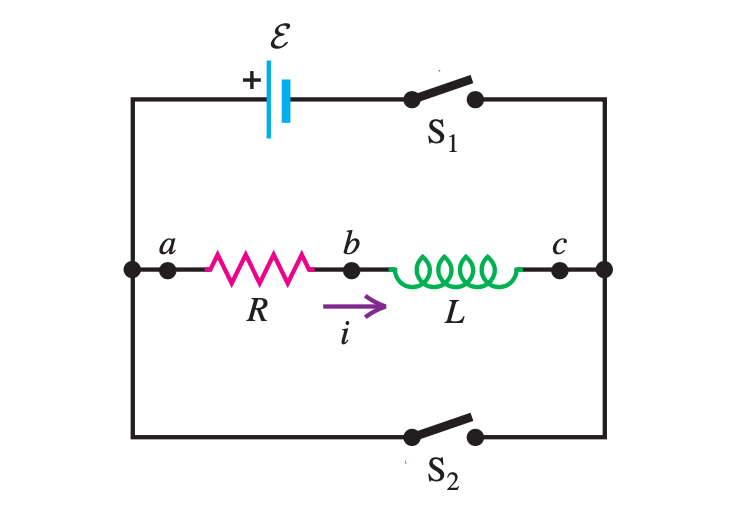
\includegraphics[scale=0.4]{fig/circuito2}
\caption{Al cerrar el interruptor $S_1$ se conecta la combinación $R-L $en serie con una fuente de fem $\varepsilon$. Al cerrar el interruptor $S_2$ al mismo tiempo que se abre $S_1$ se desconecta la combinación de la fuente.}
\end{figure}

Un circuito que incluye tanto un resistor como un inductor, y tal vez una fuente de fem, se llama circuito $R_L$ (figura \ref{fig:circuito2}).  El inductor ayuda a impedir los cambios rápidos en una corriente, lo que puede ser útil si se requiere una corriente estable y la fuente externa tiene una fem fluctuante.







%\end{document}
